\part{Passado, Presente e Futuro}
\label{ch:capitulo9}
\chapter*{Passado, Presente e Futuro}

Agora, munidos da compreensão da rede Bitcoin como um todo, podemos examinar alguns comportamentos interessantes que surgiram nos últimos dez anos do sistema.

\paragraph{ASICs e pools de mineração}
\paragraph{}

No início, Satoshi minerou os primeiros bitcoins usando a unidade de processamento central (CPU) do computador. Como a dificuldade inicial de mineração no sistema era baixa, era relativamente barato gerar essas moedas usando a CPU.

Com o tempo, as pessoas começaram a ajustar o software de mineração para torná-lo cada vez mais eficiente. Eventualmente, eles escreveram um software que começou a tirar proveito de processadores especializados chamados unidades de processamento gráfico (GPUs) que existem nas placas de vídeo e geralmente são usados para jogos.

Com as GPUs, a mineração tornou-se milhares de vezes mais eficiente do que a mineração usando a CPU. Nesse ponto, qualquer pessoa que minerava em uma CPU fornecia uma fração tão pequena da taxa de hash que rapidamente se tornou inútil, pois a dificuldade aumentou devido a todos os novos mineradores de GPU.

Conforme as GPUs assumiram o controle e as pessoas começaram a comprar toneladas de placas gráficas, a eficiência da mineração foi aprimorada ainda mais por meio da produção de ASICs (Application Specific Integrated Circuits, ou Circuitos Integrados Específicos de Aplicações em português). São chips de hardware de computador que são criados com um objetivo específico - a função bitcoin sha256 e nada mais. Sendo especializados neste algoritmo em particular, os ASICs foram capazes de ser milhares de vezes mais eficientes do que as GPUs para mineração e rapidamente tornaram as GPUs não lucrativas, assim como as GPUs fizeram com as CPUs. Em poucos anos, a nova geração de dispositivos ASIC coloca suas versões anteriores fora do mercado com grandes melhorias de eficiência.

Os primeiros mineradores da rede gastaram apenas alguns centavos de eletricidade para produzir seus bitcoins. À medida que o preço do bitcoin subia e mais e mais mineradores aderiam a rede, a dificuldade aumentava e ficava cada vez mais caro gerar bitcoins.

Um problema com a mineração de bitcoin é que ela não é determinística, como jogar um dado. Isso significa que você pode acabar gastando centenas de dólares em eletricidade e nunca encontrar um bloco válido.

Em 2010, uma inovação chamada pool de mineração (conhecida como Slushpool) surgiu para resolver o problema de mineradores consumindo energia sem receber recompensa. Um pool de mineração é um pool de risco compartilhado, semelhante ao funcionamento do seguro médico.

Todos os mineradores contribuem com a mineração, fazendo com que todos os participantes pareçam um grande mineirador. Se alguém na pool encontrar um bloco válido, a recompensa pelo bloco é dividida proporcionalmente entre todos os mineradores com base na taxa de hash com que contribuíram. Isso permite que até mesmo pequenas operações de mineração, como indivíduos, recebam recompensa pela pequena taxa de hash com que contribuem. Para fornecer este serviço de coordenação, o pool fica com uma parte das recompensas.
\newpage
Os pools de mineração causaram um efeito de centralização, os usuários migraram para pools maiores. O diagrama abaixo mostra a distribuição aproximada da mineração em janeiro de 2019.

\begin{figure}
  \centering
  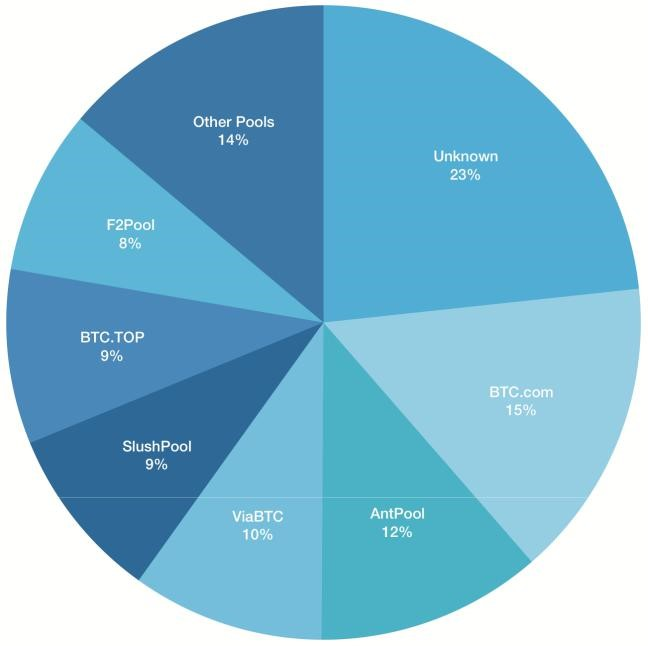
\includegraphics[width=7cm]{imagens/capitulo-9-pizza.jpg}
  \caption{Pools de mineração}
\end{figure}

\paragraph{Ataques de 51\%}
\paragraph{}

A centralização do pool de mineração leva à preocupação de que eles possam conspirar para o ataque de 51\% da rede. Se você olhar o gráfico acima, verá que as 5 principais pools, em conjunto, têm mais de 50\% da taxa de hash de mineração total.

Vamos examinar como esse ataque é realizado e quais perigos ele carrega.

Quando você possui pouco mais de 50\% da taxa de hash, pode dominar as gravações no livro-razão porque pode produzir uma cadeia mais longa do que a outra taxa de hash inferior a 50\% combinada ao longo do tempo. Lembre-se de que o Consenso de Nakamoto diz que os nodes devem aceitar a cadeia de Prova de Trabalho cumulativa mais longa que chegar até eles.

Aqui está um exemplo de como um ataque simples de 51\% é realizado:

\begin{enumerate}
\item Digamos que a rede como um todo esteja produzindo 1000 hashes/segundo;
\item Você compra um monte de hardware de mineração e eletricidade para produzir 2.000 hashes/segundo. Agora você tem 66\% da taxa total de hash (2000/3000);
\item Você começa a minerar uma cadeia que contém apenas blocos vazios;
\item Daqui a duas semanas, você transmitirá sua blockchain vazia. Como você está minerando aproximadamente duas vezes mais rápido que os mineradores honestos, sua cadeia será duas vezes mais longa focando na Prova de Trabalho cumulativa. A transmissão para todos os nodes existentes fará com que eles se reorganizem e percam as últimas duas semanas de história escrita na blockchain.
\end{enumerate}

Além de minerar blocos vazios, o que torna a blockchain inutilizável, você também pode realizar um ataque de gasto duplo:

\begin{enumerate}
\item Envie algum bitcoin para uma exchange;
\item Troque por USD e retire o USD;
\item Mais tarde, transmita na blockchain que você minerou secretamente e que não contém o envio para a exchange;
\item Você reescreveu a história e agora tem o bitcoin original e os dólares;
\end{enumerate}

Na prática, com a taxa de hash do Bitcoin hoje (lembre-se, ele está usando a mesma quantidade de energia de um país de porte médio), adquirir hardware e eletricidade suficientes para realizar tal ataque é extremamente caro. Também é muito difícil escapar impune com um ataque de gasto duplo dessa proporção sem deixar pegadas que poderiam ser usadas para descobrir quem você é. Afinal, você estaria consumindo a energia de um país de porte médio e comprando milhões de dólares em hardware e enviando milhões de dólares para a exchange para fazer todo este processo.

Manter esse tipo de ataque por qualquer período de tempo razoável é inviável, e se alguma entidade mal-intencionada com financiamento ilimitado decidisse fazer isso e fosse capaz de sustentar esse ataque além do nível de um incômodo, a rede poderia se adaptar alterando a sua função de prova de trabalho (usando alguma coisa diferente do sha256), que tornaria todos os ASICs de hardware usados pelo invasor completamente inúteis. Essa, no entanto, é a opção nuclear, pois também tiraria do mercado imediatamente todos os mineradores honestos. No entanto, a rede sobreviveria e surgiria das cinzas, como a Fênix.

Além da inviabilidade do ataque, ter a maioria da taxa de hash não dá direito a ser dono da rede:

\begin{enumerate}
\item Você não pode criar moedas do nada. Isso viola a regra de consenso de recompensa de blocos, sendo eles rejeitados, mesmo se tivessem Prova de Trabalho suficiente;
\item Você não pode gastar moedas que não são suas. Você não seria capaz de fornecer uma assinatura digital válida, o que viola as regras;
\item Você não pode acelerar o cronograma de emissão de Bitcoin. A dificuldade seria ajustada a cada 2016 blocos como sempre faz.
\end{enumerate}

Assim, os nodes que aceitam Bitcoin como pagamento manteriam a rede honesta mesmo em face de uma maioria desonesta de mineradores. Além disso, não devemos presumir que, apenas porque um pool de mineração tem uma porcentagem específica de taxa de hash, eles possuem o hardware. Na verdade, a maioria das pools de mineração é composta por milhares de mineradores individuais. Se o pool de mineração começar a se comportar mal, esses mineradores teriam um incentivo para sair do pool porque gostariam de proteger o valor econômico do Bitcoin, que estão minerando presumivelmente para ganhar dinheiro e não para ter prejuízos!

Na verdade, há um precedente histórico para mineradores individuais deixarem uma pool que se tornou muito poderosa: em 2014, a Ghash.io tinha quase metade do poder de mineração total. Os mineiros viram que ele estava se tornando muito centralizada e partiram para outras pools de maneira voluntaria.

Embora pools de mineração relativamente centralizadas sejam a realidade atual, há melhorias constantes na tecnologia de mineração, incluindo uma proposta chamada BetterHash, que permite que os mineradores individuais tenham mais controle sobre o que estão minerando e reduza a dependência da coordenação das pools.

\paragraph{Hard Forks e Soft Forks}
\paragraph{}

Deixamos o tópico mais complexo do Bitcoin para o final.

Esperamos que agora você tenha um bom controle sobre como o software Bitcoin impõe as regras que as pessoas concordaram e como as pessoas podem decidir qual software executar para aplicar as regras em que acreditam.

Também falamos que os mineradores decidem as regras que seguirão ao produzir blocos e que devem minerar o tipo de blocos que os usuários desejam, ou arriscar que seus blocos não sejam aceitos e, assim, perder a recompensa da mineração.

Finalmente, sabemos que o software do Bitcoin aceitará a mais longa cadeia de prova cumulativa de trabalho como sendo a blockchain válida, e que forks (ou bifurcações em português), às vezes, ocorrem naturalmente devido à mineração dos mineradores usando as cadeias desatualizadas.

Agora vamos falar sobre forks intencionais. Um fork intencional é quando alguns usuários e/ou mineradores decidem que não concordam com as regras atuais do Bitcoin e que precisam mudar as regras. Existem dois tipos de forks, que mudam as regras que foram definidas anteriormente: soft forks, que são compatíveis com versões anteriores, e hard forks, que não são compatíveis com versões anteriores. Vamos ver como isso ocorre na teoria e, em seguida, ver alguns exemplos históricos.

\paragraph{Soft Forks}
\paragraph{}

Um soft fork é uma mudança compatível com as regras de consenso do Bitcoin. O que isso significa? Isso significa que se você executar um node antigo que não foi atualizado para as novas regras, ele ainda verá os blocos produzidos sob as novas regras como válidos. Para um node atualizado com o novo software soft fork, todos os blocos que eram anteriormente inválidos permanecem inválidos, mas alguns blocos válidos agora são considerados inválidos. Vejamos um exemplo para deixar claro:

Em 12 de setembro de 2010, uma nova regra foi introduzida no software: Os blocos devem ter no máximo 1 MB de tamanho. Esta regra foi introduzida para resolver problemas de spam na blockchain. Antes dessa regra, todos os blocos de qualquer tamanho eram válidos. Com a nova regra, apenas blocos menores eram válidos. Se você estava executando um node antigo e não o atualizou, os blocos menores ainda eram válidos de acordo com suas regras, então você não foi afetado.

Um soft-fork é uma maneira de atualizar o sistema sem interrupções porque permite que os operadores dos nodes atualizem para o novo software lentamente ao longo do tempo, de forma voluntária. Se eles não fizerem a atualização, eles ainda serão capazes de processar todos os blocos que chegam como sempre fizeram. Apenas os  mineradores que produzem os blocos precisam se atualizar para começar a produzir blocos usando as novas regras. Depois que os mineradores atualizaram para o novo fork de 1 MB, todos os blocos daquele ponto em diante tinham no máximo 1 MB de tamanho. Os usuários que executam versões antigas do software não precisavam saber disso.


\paragraph{Hard Forks}
\paragraph{}

Um hard fork é o oposto de um soft fork. No caso de um hard fork, uma alteração não compatível com versões anteriores é introduzida na qual os blocos que eram originalmente inválidos agora são considerados válidos. No caso de um hard fork, os nodes antigos que não foram atualizados não serão capazes de processar os blocos produzidos sob as novas regras. Assim, eles ficarão presos na blockchain antiga, a menos que façam a atualização. Um exemplo de hard fork seria aquele que alterasse o tamanho do bloco de 1 MB para algo maior, pois os blocos seriam inválidos de acordo com as regras antigas.

A maioria dos hard forks com concordância quase unânime de todos os nodes da rede não causaria problemas. Cada node seria atualizado imediatamente para as novas regras. Se alguns retardatários fossem deixados para trás, eles não obteriam novas atualizações de bloco e consequentemente notariam que seu software parou de funcionar e seriam forçados a atualizá-los.

Na prática, os hard forks nunca são feitos de maneira suave. Em um sistema anárquico verdadeiramente descentralizado, você não pode coagir todos a mudarem para as novas regras. Em agosto de 2017, algumas pessoas que não estavam felizes com o progresso da rede Bitcoin em relação a pagamentos baratos decidiram que queriam fazer um fork para criar uma rede com blocos maiores. Como o Bitcoin tinha uma regra sobre os blocos não ultrapassarem 1 MB (devido a um soft fork ocorrido em 2010), essas pessoas queriam criar uma nova cadeia com blocos maiores. Este fork ficou conhecido como Bitcoin Cash.

Um hard fork fora do consenso como Bitcoin Cash, que não é seguido por todos os mineradores e nodes, cria uma nova blockchain que compartilha alguma história com a blockchain original, mas a partir do ponto de divisão em diante, as moedas criadas no fork não são mais Bitcoin, pois não são aceitas por nenhum node da rede Bitcoin.

O assunto o que “é” ou “não é” Bitcoin foi calorosamente debatido no ano seguinte ao fork do Bitcoin Cash. Houve algumas pessoas em favor do Bitcoin Cash que propuseram uma narrativa de que o Bitcoin deve ser definido pelo que está escrito no white paper original, escrito por Satoshi há dez anos, escolhendo a dedo as palavras específicas no documento para provar seu ponto. Mas um sistema baseado em consenso não funciona com base em argumentos feitos nas redes sociais. Funciona por pessoas que optam por executar um software específico para fazer cumprir regras específicas.

No caso deste fork, as pessoas que executam a grande maioria dos nodes economicamente significativos - ou seja, carteiras, exchanges e comerciantes não queriam trocar seu software por algo suportado por uma equipe de desenvolvimento muito menor e menos experiente e em uma quantidade muito menor de hash que sinalizou que eles queriam mudar para essas regras. Nem as pessoas achavam que tal “atualização” valesse a pena quando comparado a possibilidade de interrupção do ecossistema. O problema com os hard forks é que eles só funcionam quando todos aceitam a troca. Se houver retardatários, duas moedas são criadas. Assim, o Bitcoin permaneceu como sendo o Bitcoin e o Bitcoin Cash tornou-se uma moeda separada.

Hoje, existem dezenas de outros forks de Bitcoin, como Bitcoin Gold, Bitcoin Diamond e Bitcoin Private, com um pequeno hash protegendo-os, baixo suporte ao desenvolvedor e atividade econômica quase inexistente. Muitos são golpes ou projetos de pesquisa mal elaborados. Centenas de moedas semelhantes ao Bitcoin usam código semelhante, mas não compartilham o histórico de saldo da conta do Bitcoin (conjunto UTXO), como Litecoin ou Dogecoin.

\paragraph{O Livre Mercado}
\paragraph{}

Mencionamos brevemente as taxas de transação no Capítulo 5 ao discutir a mineração, mas elas merecem sua própria seção. Uma vez que a programação de emissão de Bitcoin consiste em halvings acontecendo a cada quatro anos, até que a Recompensa de Bloco seja totalmente eliminada e o Bitcoin entre em um estado de cunhagem zero até o fim dos tempos, ainda precisamos de uma forma de incentivar os mineradores a continuarem protegendo a rede .

As taxas são determinadas por um sistema de livre mercado, no qual os usuários pagam por espaço escasso em um bloco. Os usuários que enviam transações indicam quanta taxa estão dispostos a pagar aos mineradores, e eles podem ou não incluir as transações que são informadas, dependendo do quanto irão ganhar. Quando há poucas transações esperando para entrar no próximo bloco, as taxas tendem a ser muito baixas, pois não há competição. À medida que o espaço do bloco é preenchido, os usuários estão dispostos a pagar taxas mais altas para que suas transações sejam confirmadas rapidamente (no próximo bloco). Aqueles que não querem pagar, podem sempre definir taxas baixas e esperar mais para serem minerados em um momento com baixa demanda, quando o espaço do bloco estiver mais disponível.

Ao contrário dos sistemas financeiros tradicionais, onde as taxas tendem a se basear em uma porcentagem do valor que está sendo transferido, no Bitcoin o valor transferido não tem relação com as taxas. Tornamos as taxas proporcionais ao recurso escasso que consomem: espaço em bloco. Portanto, as taxas são medidas em satoshis por byte (bytes são 8 bits, basicamente apenas uma medida de quantos dados há em sua transação). Assim, uma transação que envia um milhão de bitcoins de um endereço para outro pode ser mais barata do que uma que consolida 1 bitcoin espalhado por 10 contas, porque o último requer mais espaço de bloco.

No passado, houve períodos em que o Bitcoin tinha uma demanda muito alta, como o que aconteceu no final de 2017, onde as taxas se tornaram extremamente altas. Desde então, alguns novos recursos foram implementados para reduzir a pressão sobre as taxas na rede.

Um deles é chamado de Segregated Witness (ou Testemunha Segregada), que reorganizou como os dados do bloco são representados separando as assinaturas digitais dos dados da transação, criando mais espaço para esses dados. As transações que tiram proveito desta atualização podem usar mais do que o 1 MB original do espaço do bloco por meio de alguns truques inteligentes que estão além do escopo deste livro.

O outro alívio para as taxas veio através do batching: As exchanges e outros participantes de alto volume no ecossistema começaram a combinar transações de bitcoin para vários usuários em uma transação. Ao contrário de um pagamento tradicional em seu banco ou PayPal que é feito de uma pessoa para outra, uma transação de Bitcoin pode combinar um grande número de entradas e produzir um grande número de saídas. Assim, uma exchange que precisa enviar bitcoin para saque para 100 pessoas pode fazê-lo em uma única transação. Este é um uso muito mais eficiente do espaço do bloco, transformando o que é ostensivamente apenas um punhado de transações de bitcoin por segundo em milhares de pagamentos por segundo.

A Segregated Witness e o batching já fizeram um trabalho muito bom na redução da demanda por espaço em bloco. Outras melhorias estão em andamento para tornar o uso do espaço do bloco mais eficiente. No entanto, chegará um momento em que as taxas de Bitcoin ficarão altas novamente, à medida que os blocos ficarem cada vez mais cheios devido à demanda.
 
\paragraph{Desenvolvimentos futuros no Bitcoin}
\paragraph{}

Neste ponto, já passamos por toda a questão de \textit{inventar o Bitcoin} e cobrimos como a rede evoluiu ao longo do tempo. Agora olhamos para o futuro e cobrimos algumas das melhorias de curto prazo que virão para o Bitcoin.

Ao contrário de uma moeda tradicional, que é algo que é impresso e usado, o Bitcoin é uma camada de dinheiro programável sobre a qual podemos construir muitos serviços. Este é um conceito totalmente novo e estamos apenas começando a ter conhecimento do que é possível ser feito.

\paragraph{Lightning Network}
\paragraph{}

Como discutimos acima, o Bitcoin teve problemas com taxas altas à medida que o espaço em bloco se tornou cada vez mais procurado. Hoje, o Bitcoin é capaz de apenas cerca de 3 a 7 transações por segundo com base no número de transações que cabem em um bloco. Lembre-se que cada transação pode, na verdade, ser um pagamento para centenas de pessoas por lote. Ainda assim, não tem a capacidade suficiente para se tornar uma rede global de pagamentos.

Uma solução ingênua pode ser aumentar o tamanho do bloco, e de fato várias moedas concorrentes, incluindo o Bitcoin Cash, tentaram essa abordagem. O Bitcoin não segue esse caminho porque aumentar o tamanho do bloco impactaria negativamente as características de descentralização, como o número de nodes e a dispersão geográfica. Mesmo que um aumento no tamanho do bloco fosse possível devido a melhorias no hardware, há também o problema de que a natureza descentralizada do Bitcoin significa que um hard fork que tenta mudar o tamanho do bloco causaria muitos problemas, e provavelmente ocorreria outra divisão da blockchain, criando assim, uma moeda diferente.

Um aumento no tamanho do bloco também não resolveria o problema de tornar o Bitcoin adequado como um sistema de pagamento mundial - ele simplesmente não seria tão escalável. É aqui que entra a Lightning Network: Outro protocolo e conjunto de implementações de software que criam transações offchain de Bitcoins.
 
The Lightning Network pode ser o assunto de todo um livro, mas vamos discuti-la brevemente.

A ideia da Lightning é que nem todas as transações precisam ser registradas na blockchain. Por exemplo, se você e eu estamos em um bar comprando bebidas, podemos abrir uma conta no bar e resolver no final da noite. Realmente não faz sentido cobrarmos de nosso cartão de crédito por cada bebida, pois é uma perda de tempo. Com o Bitcoin, usar a energia equivalente à de um país inteiro ao confirmar a compra de um café ou cerveja e ter essa compra registrada o tempo todo em milhares de computadores em todo o mundo não é escalonável nem particularmente bom para a privacidade.

A Lightning Network, se for bem-sucedida, melhorará muitas das desvantagens do Bitcoin:

\begin{enumerate}
\item Transferência de transações virtualmente ilimitada. Centenas de milhares de micro transações poderiam ser realizadas usando a blockchain Bitcoin uma vez, como liquidação final;
\item Confirmações instantâneas; não há necessidade de esperar que os blocos sejam minerados;
\item Taxas de transação de menos de um centavo adequadas para micro pagamentos, como pagar um centavo para ler um blog;
\item Maior privacidade. Apenas as partes que participam da transação precisam saber sobre ela, ao contrário de uma transação em rede que é transmitida para o mundo inteiro.
\end{enumerate}

A Lightning usa o conceito de canais de pagamento, que são transações reais de Bitcoin na blockchain que bloqueiam uma certa quantidade de Bitcoin e o tornam disponível na Lightning Network para transferência instantânea e quase gratuita. A Lightning Network está nos estágios iniciais, mas já se mostra promissora. Você pode verificar o site \textit{\url{https://yalls.org/}} que usa micro pagamentos baseados na Lightning para disponibilizar a leitura de artigos.

\paragraph{Bitcoin no Espaço}
\paragraph{}

O Bitcoin faz um excelente trabalho de ser resistente à censura, pois é resistente ao confisco (você pode carregá-lo em sua cabeça) e resistente à censura de transferência, uma vez que requer apenas um minerador honesto na rede para garantir suas transações (e você pode minerar você mesmo).

No entanto, sendo o Bitcoin transmitido pela Internet, é suscetível de censura em nível de rede. Os regimes autoritários que querem reprimir a atividade podem tentar bloquear o tráfego de Bitcoin que entra e sai de seu país.

O Blockstream Satellite é o primeiro esforço para contornar a censura de rede em nível estadual, bem como alcançar áreas remotas que podem não ter conexões com a Internet. Este satélite permite que qualquer pessoa com uma antena parabólica e equipamento relativamente barato conecte e baixe a blockchain do Bitcoin, com comunicação bidirecional em breve. Agora também existem esforços como o TxTenna para construir redes fora da grade elétrica. Quando acoplado a uma conexão via satélite, esse tipo de configuração seria quase imparável\footnote{Nota do tradutor: Atualmente um grupo de brasileiros usou ondas de rádio para colocar uma transação na rede usando a Lua como ponto de reflexo. Veja mais em \url{https://livecoins.com.br/brasileiros-enviam-bitcoin-a-lua-na-frente-de-elon-musk/}}.